\documentclass[margin=2cm]{standalone}
%\usepackage{amssymb}		need this for \varnothing
\usepackage{tikz}
\usetikzlibrary{calc,intersections,through,backgrounds,patterns}

%adapted from https://tex.stackexchange.com/questions/349524/how-to-draw-this-complex-simplex
%payoffs come from Ferguson (2014: 25) -- http://www.math.ucla.edu/~tom/Game_Theory/coal.pdf

\begin{document}

%$v(\{A\}) = -1$ 	$v(\{AB\}) = 3$ 	$v(\{N\}) = 5$
%$v(\{B\}) =  0$ 	$v(\{AC\}) = 4$ 	$v(\{\varnothing\}) = 0$
%$v(\{C\}) =  1$ 	$v(\{BC\}) = 2$

%The imputations are the points $(x_1, x_2, x_3)$ such that $x_1 + x_2 + x_3 = 5$ and $x_1 \geq -1$, $x_2 \geq 0$, $x_3 \geq 1$. These form a triangle with vertices (4,0,1), (-1,5,1), and (-1,0,6), where two players get their minimums and the third gets the rest.

%Since $\{A,B\}$ can guarantee itself $v(\{AB\}) = 3$ all points with $x_1 + x_2 < 3$ are unstable through $\{A,B\}$. Likewise, all points with $x_1 + x_3 < 4$ are unstable through $\{A,C\}$, and all points with $x_2 + x_3 < 2$ are unstable through $\{B,C\}$.

%Hence, we can identify the core by plotting the simplex diagram.

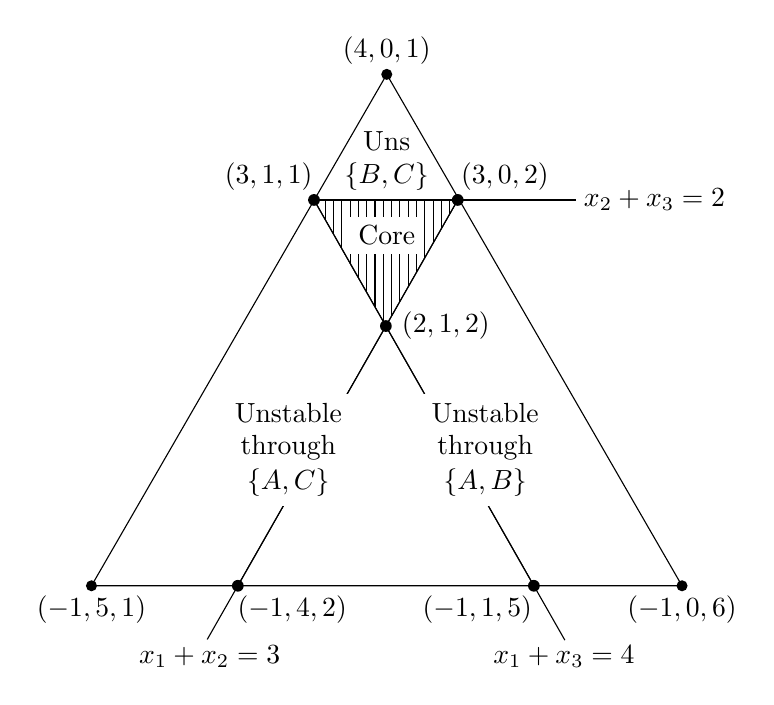
\begin{tikzpicture}
\coordinate (A) at (0,0);
\coordinate (B) at (7.5,0);
\draw (A)node[below]{$(-1,5,1)$} -- (B)node[below]{$(-1,0,6)$} --++ (120:7.5)coordinate(C)node[above]{$(4,0,1)$} -- cycle;
\fill (A) circle (2pt);\fill (B) circle (2pt);\fill (C) circle (2pt);
%
\draw [name path=parallel](2.75,4.9)coordinate(Ap)--(6.15,4.9)coordinate(Bp); %horizontal line: 
%
\draw[name path=B--C] ($(B)!0.05!(C)!16.5mm!98:(C)$)coordinate(X1) -- ($(B)!0.935!(C)!16.5mm!104.5:(C)$)coordinate(X2); %top-to-bottom, left-to-right
%
\draw[name path=C--A] ($(C)!0.05!(A)!16.5mm!73:(A)$)coordinate(X3) -- ($(C)!0.935!(A)!16.5mm!78:(A)$)coordinate(X4); %top-to-bottom, right-to-left
%
\path [name intersections={of=parallel and B--C,by=E}];
\path [name intersections={of=parallel and C--A,by=F}];
\node [fill=black,circle,inner sep=1.5pt] at (E) {};
\node [fill=black,circle,inner sep=1.5pt] at (F) {};
\draw [name path=A--B] (A)--(B);
\path [name intersections={of=B--C and A--B,by=G}];
\node [fill=black,circle,inner sep=1.5pt] at (G) {};
\path [name intersections={of=C--A and A--B,by=H}];
\node [fill=black,circle,inner sep=1.5pt] at (H) {};
%
\draw [name path=E--G] (E)--(G);
\draw [name path=F--H] (F)--(H);
\path [name intersections={of=E--G and F--H,by=I}];
\node [fill=black,circle,inner sep=1.5pt] at (I) {};
%
\node at (2.25,5.2) {$(3,1,1)$};
\node at (5.25,5.2) {$(3,0,2)$};
\node at (4.5,3.3) {$(2,1,2)$};
\node at (2.55,-0.3) {$(-1,4,2)$};
\node at (4.9,-0.3) {$(-1,1,5)$};
\node at (7.15,4.9) {$x_2 + x_3 = 2$};
\node at (1.5,-0.9) {$x_1 + x_2 = 3$};
\node at (6,-0.9) {$x_1 + x_3 = 4$};
%
\path[pattern=vertical lines,pattern color=black] (E)--(F)--(I)--cycle;
\node [fill=white] at (3.75,4.45) {Core};
%
\node [fill=white] at (2.5,2.2) {Unstable};
\node [fill=white] at (2.5,1.75) {$\;$through$\;$};
\node [fill=white] at (2.5,1.31) {$\;\;\{A,C\}\;\;$};
%
\node [fill=white] at (5,2.2) {Unstable};
\node [fill=white] at (5,1.75) {$\;$through$\;$};
\node [fill=white] at (5,1.31) {$\;\;\{A,B\}\;\;$};
%
\node at (3.75,5.65) {Uns};
\node at (3.75,5.2) {$\{B,C\}$};
\end{tikzpicture}

\end{document}